\documentclass[aspectratio=169,10pt]{beamer}

\usetheme{metropolis}
\usepackage{appendixnumberbeamer}
\usepackage{booktabs}
\usepackage[scale=2]{ccicons}
\usepackage{pgfplots}
\usepgfplotslibrary{dateplot}
\usepackage{xspace}
\usepackage{graphicx}
\usepackage{tikz}
\usetikzlibrary{mindmap,trees,shapes,arrows,pie}
\usepackage{tcolorbox}

\newcommand{\themename}{\textbf{\textsc{metropolis}}\xspace}

\title{Navigating the PhD Landscape in Europe and Germany}
\subtitle{Session 1: Embarking on Your Doctoral Journey}
\date{\today}
\author{Dr. Bijun Li}
\institute{Expert in International Academic Environments}

\begin{document}

\maketitle

\begin{frame}{Series Overview}
    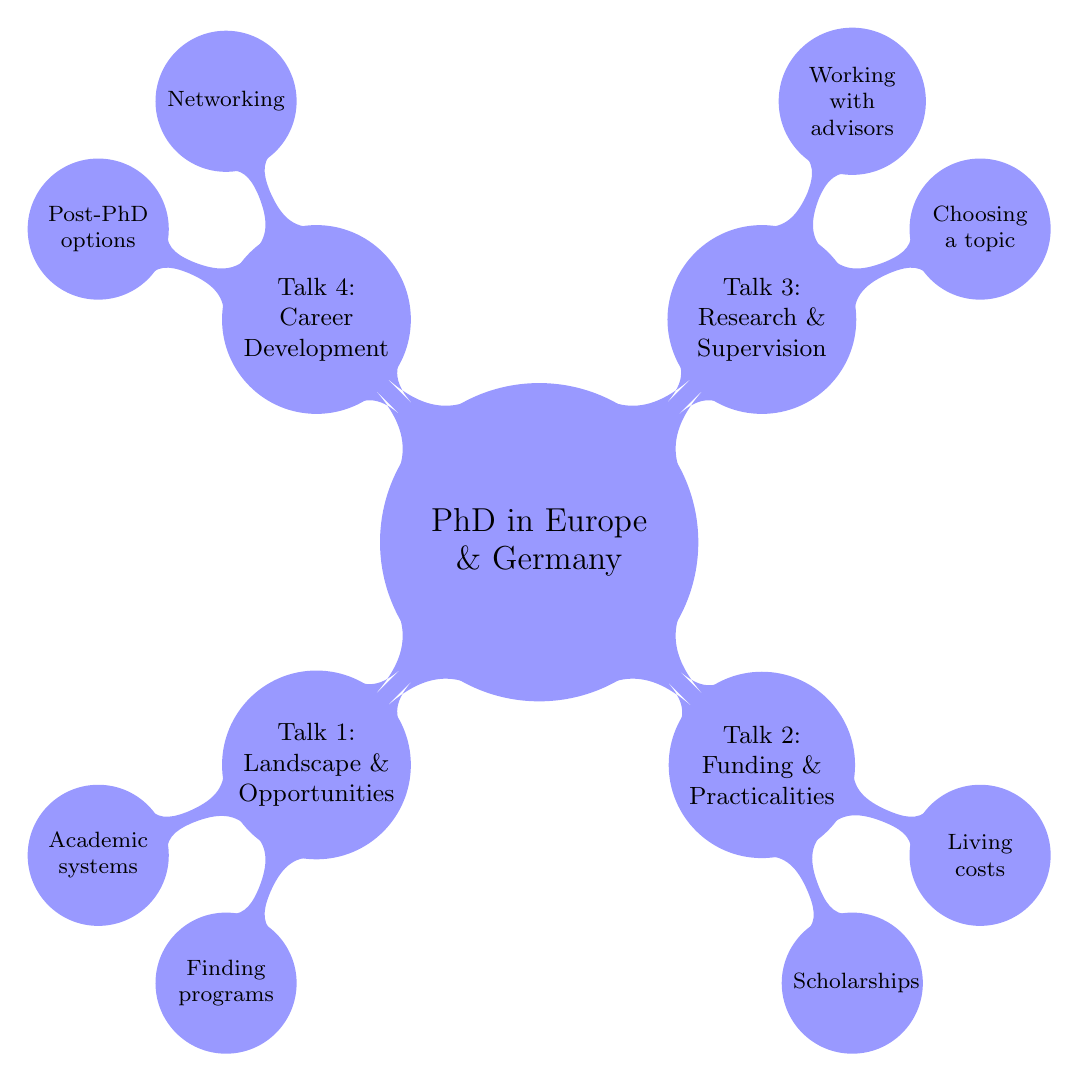
\begin{tikzpicture}[mindmap, grow cyclic, every node/.style=concept, concept color=blue!40,
                        level 1/.append style={level distance=4cm,sibling angle=90},
                        level 2/.append style={level distance=3cm,sibling angle=45}]
        
        \node{PhD in Europe \& Germany}
        child { node {Talk 1: Landscape \& Opportunities}
            child { node {Academic systems} }
            child { node {Finding programs} }
        }
        child { node {Talk 2: Funding \& Practicalities}
            child { node {Scholarships} }
            child { node {Living costs} }
        }
        child { node {Talk 3: Research \& Supervision}
            child { node {Choosing a topic} }
            child { node {Working with advisors} }
        }
        child { node {Talk 4: Career Development}
            child { node {Networking} }
            child { node {Post-PhD options} }
        };
    \end{tikzpicture}
\end{frame}

\begin{frame}{Learning Objectives for Today}
    By the end of this session, you will be able to:
    \begin{itemize}
        \item Understand the structure of PhD programs in Europe, with a focus on Germany
        \item Navigate the diverse European doctoral landscape
        \item Identify key differences in the German academic ecosystem
        \item Develop strategies for finding PhD opportunities
        \item Craft effective communications with potential supervisors
        \item Begin building your academic network
    \end{itemize}
\end{frame}

\begin{frame}{About Your Guide}
\begin{columns}[T]
    \begin{column}{0.7\textwidth}
        \begin{itemize}
            \item Dr. Bijun Li, PhD in Computer Science from Technical University of Munich
            \item Specialization: Machine Learning for Climate Modeling
            \item Current role: Postdoctoral Researcher at Max Planck Institute for Meteorology
            \item 5+ years of experience in international academic settings
            \item Published in top-tier journals: Nature Climate Change, Journal of Climate
            \item Personal experience: Moved from China to Germany for PhD studies
        \end{itemize}
    \end{column}
    \begin{column}{0.3\textwidth}
%        \includegraphics[width=\textwidth]{/api/placeholder/200/200}
%        \caption*{Dr. Bijun Li}
    \end{column}
\end{columns}
\end{frame}

\begin{frame}{Why This Series Matters}
\begin{columns}[T]
    \begin{column}{0.6\textwidth}
        \textbf{Benefits of a PhD in Europe/Germany}
        \begin{itemize}
            \item World-class research facilities
            \item Strong industry collaborations
            \item Multicultural academic environment
            \item Generally tuition-free programs
            \item Opportunities for EU-wide mobility
        \end{itemize}
    \end{column}
    \begin{column}{0.4\textwidth}
        \textbf{International PhD Students in Germany (2020)}
        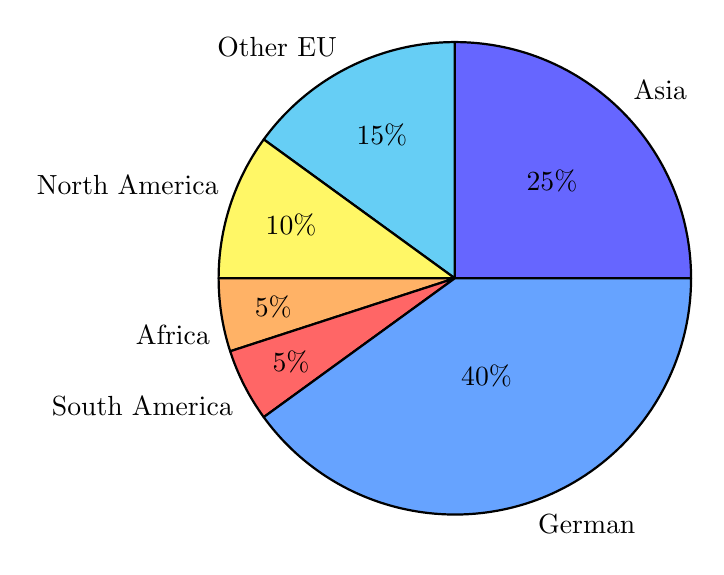
\begin{tikzpicture}
            \pie{25/Asia, 15/Other EU, 10/North America, 5/Africa, 5/South America, 40/German}
        \end{tikzpicture}
        \tiny{Source: DAAD, 2021}
    \end{column}
\end{columns}
\end{frame}

\begin{frame}{European PhD Landscape}
\begin{columns}[T]
    \begin{column}{0.5\textwidth}
        \textbf{Bologna Process Impact}
        \begin{itemize}
            \item Standardized 3-cycle system (Bachelor, Master, Doctorate)
            \item Enhanced mobility within Europe
            \item Focus on quality assurance
            \item Introduction of ECTS credits
        \end{itemize}
    \end{column}
    \begin{column}{0.5\textwidth}
        \textbf{Comparison with Other Regions}
        \begin{tabular}{|l|c|c|c|}
        \hline
        Aspect & Europe & US & Asia \\
        \hline
        Duration & 3-4 years & 5-7 years & 3-5 years \\
        Coursework & Limited & Extensive & Varied \\
        Funding & Often employed & Often TA/RA & Varied \\
        \hline
        \end{tabular}
    \end{column}
\end{columns}
\end{frame}

\begin{frame}{German Academic Ecosystem}
\begin{columns}[T]
    \begin{column}{0.5\textwidth}
        \textbf{Types of Institutions}
        \begin{itemize}
            \item Universities (Universitäten)
            \item Universities of Applied Sciences (Fachhochschulen)
            \item Research Institutes (e.g., Max Planck, Fraunhofer)
        \end{itemize}
        \textbf{Excellence Initiative Impact}
        \begin{itemize}
            \item Increased international visibility
            \item Enhanced research funding
            \item Creation of "Elite" universities
        \end{itemize}
    \end{column}
    \begin{column}{0.5\textwidth}
        \textbf{Research Clusters}
        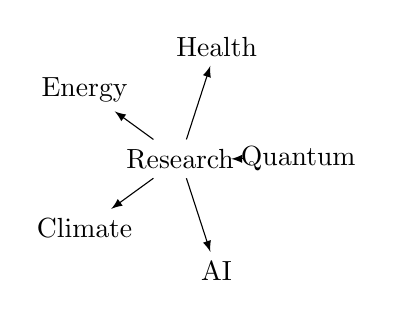
\begin{tikzpicture}[grow cyclic, ->,>=latex, level 1/.style={sibling angle=72}]
        \node[](z){Research}
          child{node[]{Climate}}
          child{node[]{AI}}
          child{node[]{Quantum}}
          child{node[]{Health}}
          child{node[]{Energy}};
        \end{tikzpicture}
    \end{column}
\end{columns}
\end{frame}

\begin{frame}{Uncovering PhD Opportunities}
\textbf{Online Resources Demo}
\begin{itemize}
    \item DAAD Database: \url{www.daad.de/deutschland/promotion/phd/en/}
    \item Research in Germany: \url{www.research-in-germany.org/en/jobs-and-careers/info-for-phd-students.html}
    \item EuroDoc: \url{www.eurodoc.net/}
\end{itemize}

\vspace{0.5cm}

\textbf{Evaluating Program Fit}
\begin{itemize}
    \item Research alignment
    \item Supervisor expertise
    \item Funding opportunities
    \item Location and facilities
    \item Career development support
\end{itemize}
\end{frame}

\begin{frame}{Approaching Potential Supervisors}
\textbf{Good Initial Contact Email}
\begin{tcolorbox}[colback=green!5,colframe=green!40!black]
Subject: Inquiry about PhD position in Machine Learning for Climate Modeling

Dear Professor [Name],

I am writing to express my interest in pursuing a PhD under your supervision...

[Brief introduction, research interests, relevant experience]

I am particularly interested in your recent work on [specific project/paper]...

[Question about current research or potential projects]

Thank you for your time and consideration.

Sincerely,
[Your Name]
\end{tcolorbox}

\textbf{Tips for Follow-up}
\begin{itemize}
    \item Be patient (wait at least 2 weeks before following up)
    \item Keep it brief and polite
    \item Reiterate your interest
    \item Offer additional information if needed
\end{itemize}
\end{frame}

\begin{frame}{Building Your Academic Network}
\textbf{Networking Opportunities in Germany}
\begin{itemize}
    \item German Physical Society (DPG) Annual Meetings
    \item Lindau Nobel Laureate Meetings
    \item CeBIT (for technology and digital business)
    \item Heidelberg Laureate Forum (for mathematics and computer science)
\end{itemize}

\vspace{0.5cm}

\textbf{Leveraging Social Media}
\begin{itemize}
    \item Twitter: Follow researchers, institutions, and relevant hashtags
    \item LinkedIn: Join groups related to your field and German academia
    \item ResearchGate: Share your work and engage in discussions
\end{itemize}
\end{frame}

\begin{frame}{Application Process for German Universities}
\textbf{Key Requirements}
\begin{itemize}
    \item Master's degree (or equivalent)
    \item Strong academic record (typically 2.5 or better in German grading system)
    \item Proof of English proficiency (often IELTS 6.5+ or equivalent)
    \item Research proposal
    \item Letters of recommendation
\end{itemize}

\vspace{0.5cm}

\textbf{Typical Timeline}
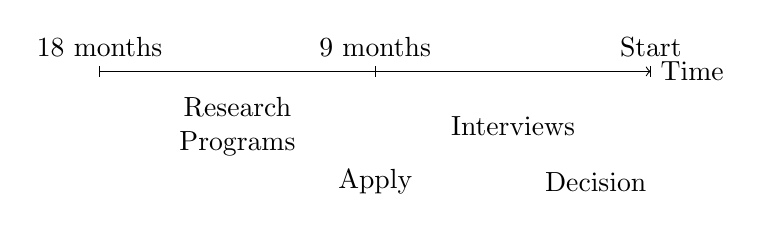
\begin{tikzpicture}[scale=0.7]
    \draw[->] (0,0) -- (10,0) node[right] {Time};
    \draw (0,-0.1) -- (0,0.1) node[above] {18 months};
    \draw (5,-0.1) -- (5,0.1) node[above] {9 months};
    \draw (10,-0.1) -- (10,0.1) node[above] {Start};
    
    \node[align=center] at (2.5,-1) {Research \\ Programs};
    \node[align=center] at (5,-2) {Apply};
    \node[align=center] at (7.5,-1) {Interviews};
    \node[align=center] at (9,-2) {Decision};
\end{tikzpicture}
\end{frame}

\begin{frame}{Q\&A Session}
\textbf{Common Questions}
\begin{itemize}
    \item Q: Do I need to speak German for a PhD in Germany?
    \item A: Not necessarily. Many programs, especially in STEM fields, are conducted in English. However, learning German can enhance your overall experience and career prospects.
    
    \item Q: How competitive are PhD positions in Germany?
    \item A: Competitiveness varies by field and institution. Generally, positions at top universities and in popular fields are highly competitive.
    
    \item Q: Can I work part-time during my PhD in Germany?
    \item A: Yes, most PhD students in Germany are employed by their university or research institute. Additional part-time work is possible within certain limits.
\end{itemize}

\centering{\large{Your questions?}}
\end{frame}

\begin{frame}{Additional Resources}
\begin{columns}[T]
    \begin{column}{0.5\textwidth}
        \textbf{German-specific Resources}
        \begin{itemize}
            \item Deutsch-Uni Online: \url{www.deutsch-uni.com}
            \item Make it in Germany: \url{www.make-it-in-germany.com}
            \item Study in Germany: \url{www.study-in-germany.de}
        \end{itemize}
    \end{column}
    \begin{column}{0.5\textwidth}
        \textbf{Cultural Adaptation}
        \begin{itemize}
            \item Goethe-Institut: \url{www.goethe.de}
            \item Deutsche Welle: \url{www.dw.com}
            \item InterNations: \url{www.internations.org}
        \end{itemize}
    \end{column}
\end{columns}
\end{frame}

\begin{frame}{Next Steps and Preview of Talk 2}
\textbf{Homework for Next Session}
\begin{itemize}
    \item Research funding options relevant to your field
    \item Draft a preliminary budget for PhD life in Germany
    \item Identify 2-3 potential supervisors and draft initial contact emails
\end{itemize}

\vspace{0.5cm}

\textbf{Preview of Talk 2: Funding, Practical Considerations, and Challenges}
\begin{itemize}
    \item Comprehensive overview of funding sources
    \item Detailed breakdown of living costs in Germany
    \item Strategies for overcoming common PhD challenges
    \item Tips for work-life balance and cultural integration
\end{itemize}
\end{frame}

\begin{frame}{Thank You!}
\begin{center}
\large{\textbf{We look forward to seeing you in Session 2!}}

\vspace{1cm}

Contact: \href{mailto:bijun.li@mpimet.mpg.de}{bijun.li@mpimet.mpg.de}

Follow for updates: @DrBijunLi
\end{center}
\end{frame}

\end{document}